\chapter{基于邻居相对表现的强化学习合作促进机制}
\label{chap:work1}

空间公共物品博弈中，合作能够增加群体的公共收益，但合作者需要承担个体成本。对于通过试错更新策略的智能体而言，一次交互所获得的奖励既取决于自身动作，也取决于所在群组的合作状况。邻居的行为及其获得的反馈能够提供额外的比较依据，但这些信息如何参与价值更新，仍然需要明确的规则。本章在个体 Q-learning 的基础上引入邻居影响（Neighbor Influence，NI）机制，研究相对表现信息对合作演化的作用。

本章对应已发表工作\cite{kang2025neighbor}。方法以综合奖励评价邻居表现，在标准时序差分更新之后，对当前已执行动作的 Q 值施加附加修正。下面依次介绍环境与学习过程、邻居影响规则，以及原研究关于影响强度、奖励组成和感知范围的实验结论。所有关于已发表结果的讨论均限定在原研究的模型及参数条件内。

\section{研究问题与方法概述}

个体强化学习通过自身交互经验估计动作价值。在本章的空间博弈环境中，这种经验反映了个体所在位置的局部交互结果，却没有直接比较其他个体在同一轮交互中的相对表现。例如，当两个邻居采用不同动作并获得不同奖励时，仅使用自身时序差分目标的更新过程，不会显式利用这两个邻居之间的表现差异。将这样的比较信息纳入学习，提供了一种连接个体经验与周围社会信息的方式。

本章关注三个相互关联的问题。首先，在保持个体价值学习过程的基础上，如何使邻居的相对表现参与 Q 值更新；其次，邻居影响与声誉奖励分别通过什么途径作用于合作；最后，在博弈交互范围固定时，扩大信息感知范围能否改善合作形成过程。相应地，实验分别改变邻居影响强度 $\kappa$、博弈收益权重 $w_P$ 和感知范围参数 $M$，并结合合作率、空间分布及更新贡献分析这些因素的作用。

NI 机制采用一个直接的启发式规则：优先参考综合奖励高于自身的最佳邻居，并根据双方动作是否一致，增加或减小自身已执行动作的 Q 值。该规则包含参考对象选择和价值修正两个环节。参考对象由邻居奖励排序确定，修正幅度由奖励优势与固定控制参数确定。智能体在下一轮仍通过自身 Q 表选择动作，因此邻居经验影响的是个体的价值判断。

这一设计同时规定了本章的信息条件。邻居动作及其综合奖励被视为可准确获得的观测，模型没有区分真实值与可能被篡改的报告值。因而，本章首先回答可靠信息条件下的合作促进问题。信息失真后应如何选择邻居、调节修正强度，将在后续工作中讨论。

\section{博弈环境与个体学习过程}
\subsection{空间结构与公共物品博弈}

考虑由 $L\times L$ 个节点组成的周期方格网络，每个节点放置一个智能体，智能体总数为 $N_{\mathrm{tot}}=L^2$。周期边界将网格两端相连，使所有节点具有相同的局部连接结构。原研究采用 $L=100$，每个智能体具有四个一阶邻居。离散时刻 $t$，智能体 $i$ 选择动作 $a_i(t)\in\{0,1\}$，其中 $0$ 表示合作（$C$），$1$ 表示背叛（$D$）。

每个公共物品博弈组由一个中心节点及其四个一阶邻居构成，组规模为 $k=5$。智能体 $i$ 参与以自身及其一阶邻居为中心的五个重叠博弈组，记这些组的集合为 $G_i$。在每个组中，合作者投入成本 $c=1$，背叛者不投入成本；总投入乘以协同因子 $r$ 后，由该组所有成员均分。设组 $g$ 内的合作者数量为 $n_C(g,t)$，则智能体 $i$ 的当轮总收益为
\begin{equation}
 P_i(t)=\sum_{g\in G_i}\left[\frac{r\,n_C(g,t)}{5}-\bigl(1-a_i(t)\bigr)\right].
 \label{eq:w1-payoff}
\end{equation}
这里的成本按参与的博弈组分别扣除。一个合作者参与五个组，当轮总成本为5；$P_i(t)$ 表示累积后的原始博弈收益，尚未经过学习奖励所需的归一化与加权处理。

\subsection{信息感知范围与声誉状态}

博弈组规定收益如何产生，感知集合规定智能体可参考哪些信息。设 $\Omega_i$ 为智能体 $i$ 的感知集合。当 $M=1$ 时，该集合包含自身与四个一阶邻居；当 $M=2$ 时，进一步纳入八个二阶邻居，即与自身的网格曼哈顿距离为2的节点。因此，$|\Omega_i|$ 分别为5和13。用于 NI 参考对象选择的候选集合记为
\begin{equation}
 \Omega'_i=\Omega_i\setminus\{i\},\qquad
 |\Omega'_i|=\begin{cases}4,&M=1,\\12,&M=2.\end{cases}
 \label{eq:w1-neighborhood}
\end{equation}
图\ref{fig:w1-neighborhood}展示了两种感知范围。感知范围的扩大增加了可获取的邻居信息，而式\eqref{eq:w1-payoff}中的五人博弈组保持不变。

\begin{figure}[htbp]
 \centering
 \begin{tikzpicture}[scale=0.82]
 \draw[gray!35,step=1] (-2.5,-2.5) grid (2.5,2.5);
 \foreach \x/\y in {2/0,-2/0,0/2,0/-2,1/1,1/-1,-1/1,-1/-1}
   \node[circle,draw,dashed,fill=white,minimum size=7mm] at (\x,\y) {2};
 \foreach \x/\y in {1/0,-1/0,0/1,0/-1}
   \node[circle,draw,fill=gray!20,minimum size=7mm] at (\x,\y) {1};
 \node[circle,draw,thick,fill=gray!55,minimum size=7mm] at (0,0) {$i$};
 \node[anchor=west,align=left,font=\small] at (3.1,1.2) {博弈组：中心 $i$ 与四个一阶邻居};
 \node[anchor=west,align=left,font=\small] at (3.1,0.2) {$M=1$：自身 $+$ 4个一阶邻居};
 \node[anchor=west,align=left,font=\small] at (3.1,-0.8) {$M=2$：再加入8个二阶邻居};
 \node[anchor=west,align=left,font=\small] at (3.1,-1.8) {参考对象：从感知集合中排除自身};
\end{tikzpicture}

 \caption{博弈交互与信息感知范围示意。中心为智能体 $i$，实线圆表示四个一阶邻居，虚线圆表示八个二阶邻居。以 $i$ 为中心的博弈组由中心和一阶邻居组成；$M=2$ 时的感知集合还包含二阶邻居。本图依据模型定义绘制，不表示实验结果。}
 \label{fig:w1-neighborhood}
\par\smallskip{\zihao{-5}\rmfamily 来源：Kang等，文献\cite{kang2025neighbor}，2025年。作者依据模型定义绘制。\par}
\end{figure}

每个智能体维护声誉 $U_i(t)$，用于记录其行为历史。初始声誉为 $U_i(0)=0$，声誉限制在 $[-U_{\max},U_{\max}]$ 内，其中 $U_{\max}=10$。合作与背叛对应的名义声誉增量为
\begin{equation}
 \Delta U_i(t)=\begin{cases}+1,&a_i(t)=0,\\-1,&a_i(t)=1,\end{cases}
 \quad
 U_i(t+1)=\operatorname{clip}\bigl(U_i(t)+\Delta U_i(t),-10,10\bigr).
 \label{eq:w1-reputation}
\end{equation}
其中，$\operatorname{clip}$ 将超出上下界的值截断。$\Delta U_i(t)$ 表示动作对应的增减信号；当声誉已经达到边界时，它不必等于截断后声誉值的实际变化。例如，声誉为10的个体继续合作，其名义增量为1，而更新后的声誉仍为10。

状态由感知集合内的平均声誉构造：
\begin{equation}
 \bar U_i(t)=\frac{1}{|\Omega_i|}\sum_{j\in\Omega_i}U_j(t),\qquad
 s_i(t)=\begin{cases}1,&\bar U_i(t)>0,\\0,&\bar U_i(t)\leq0.\end{cases}
 \label{eq:w1-state}
\end{equation}
由此得到两个离散状态，分别表示正平均声誉与非正平均声誉的局部环境。每个智能体只需维护一个 $2\times2$ 的 Q 表。该表示压缩了邻域历史信息，但不会保留各邻居的具体声誉、动作或空间排列；后续的 NI 更新为个体补充了当轮邻居相对表现的信息。

声誉在模型中具有两种不同用途：累积声誉经邻域平均后用于状态构造，动作对应的声誉增量则用于即时奖励。因而，即使不把声誉增量加入奖励，状态中仍然保留声誉信息；不能将 $w_P=1$ 解释为整个系统完全不使用声誉。

\subsection{综合奖励与标准Q-learning更新}

原始博弈收益与声誉增量的取值尺度不同。原研究先分别归一化，再构造综合奖励。沿用原文的收益归一化参数 $P_{T\min}=r-5$、$P_{T\max}=4r$，得到
\begin{equation}
 P'_i(t)=\frac{P_i(t)-r+5}{3r+5},\qquad
 \Delta U'_i(t)=\frac{\Delta U_i(t)+1}{2}.
 \label{eq:w1-normalization}
\end{equation}
对于本章讨论的 $1\leq r\leq5$ 条件，上述收益上下界分别对应合作个体周围均为背叛者以及背叛个体周围均为合作者的极端情形。声誉增量归一化后，合作对应1，背叛对应0。由此构造
\begin{equation}
 R_i(t)=w_P P'_i(t)+(1-w_P)\Delta U'_i(t),\qquad 0\leq w_P\leq1.
 \label{eq:w1-reward}
\end{equation}
当 $w_P=1$ 时，即时奖励仅包含归一化博弈收益；减小 $w_P$ 会增加合作动作所获得的直接声誉奖励。改变 $w_P$ 因此改变了智能体的学习激励，而不是改变式\eqref{eq:w1-payoff}所定义的公共收益分配规则。

智能体在状态 $s_i(t)$ 下执行动作 $a_i(t)$，获得奖励 $R_i(t)$，并在声誉更新后计算下一状态 $s_i(t+1)$。记标准时序差分误差为
\begin{equation}
 \delta_i(t)=R_i(t)+\gamma\max_{a'\in\{0,1\}}Q_i\bigl(s_i(t+1),a'\bigr)
             -Q_i\bigl(s_i(t),a_i(t)\bigr),
 \label{eq:w1-td-error}
\end{equation}
则标准更新为
\begin{equation}
 Q_i\bigl(s_i(t),a_i(t)\bigr)\leftarrow
 Q_i\bigl(s_i(t),a_i(t)\bigr)+\eta\delta_i(t),
 \label{eq:w1-q-update}
\end{equation}
其中学习率 $\eta=0.8$、折扣因子 $\gamma=0.9$。式\eqref{eq:w1-td-error}右侧的 Q 值在本次标准更新之前读取。每个智能体拥有自己的 Q 表，不在智能体之间共享或平均 Q 值。

动作采用 $\epsilon$-greedy 策略选取：以概率 $1-\epsilon(t)$ 选择当前状态下 Q 值最大的动作，以概率 $\epsilon(t)$ 在两种动作中随机选择；贪心动作并列时，原模型描述采用随机打破平局。探索率按照
\begin{equation}
 \epsilon(t+1)=\max\{\epsilon_{\min},\epsilon(t)\epsilon_{\mathrm{dcy}}\},
 \label{eq:w1-epsilon}
\end{equation}
逐步减小，其中 $\epsilon(0)=0.5$、$\epsilon_{\min}=0.01$、$\epsilon_{\mathrm{dcy}}=0.99$。保留非零探索下限意味着长期行为仍可能发生随机切换，后文讨论的稳定合作水平应理解为有限仿真中的统计表现。

\section{邻居影响机制}
\subsection{参考邻居选择与奖励优势}

标准更新之后，智能体比较自身与候选邻居的当轮综合奖励。对 $j\in\Omega'_i$，定义
\begin{equation}
 \Delta R_{ij}(t)=R_j(t)-R_i(t),\qquad
 \Delta R_{i,\mathrm{md}}(t)=
 \max\left\{0,\max_{j\in\Omega'_i}\Delta R_{ij}(t)\right\}.
 \label{eq:w1-positive-gap}
\end{equation}
仅当 $\Delta R_{i,\mathrm{md}}(t)>0$ 时存在优于自身的候选邻居，此时从集合
\begin{equation}
 j_i^*(t)\in\operatorname*{arg\,max}_{j\in\Omega'_i}R_j(t)
 \label{eq:w1-best-neighbor}
\end{equation}
中确定一个参考对象。若所有邻居的奖励均不高于自身，则该轮不进行附加修正。该条件使影响来自相对奖励优势，而不是只要存在邻居就必然调整价值。

当 $w_P<1$ 时，综合奖励同时含有收益与声誉项，参考对象因而不一定是原始博弈收益最高的邻居。只有在 $w_P=1$ 且使用相同的收益归一化时，两种排序才一致。区分这两种情况，有助于解释后文中奖励组成与 NI 机制的共同作用。

\subsection{影响强度与动作一致性修正}

为控制奖励差对附加更新的影响，原模型使用全系统的最大邻居绝对奖励差进行归一化：
\begin{equation}
 \Delta R_{\mathrm{gl}}(t)=
 \max_{k\in\mathcal V}\max_{l\in\Omega'_k}|R_l(t)-R_k(t)|+\lambda_\epsilon,
 \qquad\lambda_\epsilon=0.01,
 \label{eq:w1-global-gap}
\end{equation}
其中 $\mathcal V$ 表示所有智能体的集合。智能体 $i$ 的影响强度为
\begin{equation}
 \lambda_{i,\mathrm{NI}}(t)=\kappa\,
       \frac{\Delta R_{i,\mathrm{md}}(t)}{\Delta R_{\mathrm{gl}}(t)},\qquad\kappa\geq0.
 \label{eq:w1-ni-strength}
\end{equation}
这里将原文的个体相关量显式加上索引 $i$，以区分不同节点的更新幅度，计算规则不变。分母中的正则项避免全体奖励相同时出现除零。由于分子的正奖励差不超过分母中的全局最大绝对差，$0\leq\lambda_{i,\mathrm{NI}}(t)\leq\kappa$。这一关系给出了单次附加修正的幅度约束，但不构成整个多智能体学习过程的收敛证明。

当存在更优邻居时，根据双方当轮动作定义一致性项
\begin{equation}
 \Delta_{i,\mathrm{bh}}(t)=
 \begin{cases}+1,&a_i(t)=a_{j_i^*(t)}(t),\\-1,&a_i(t)\neq a_{j_i^*(t)}(t).
 \end{cases}
 \label{eq:w1-consistency}
\end{equation}
随后，在式\eqref{eq:w1-q-update}的基础上执行
\begin{equation}
 Q_i\bigl(s_i(t),a_i(t)\bigr)\leftarrow Q_i\bigl(s_i(t),a_i(t)\bigr)
       +\lambda_{i,\mathrm{NI}}(t)\Delta_{i,\mathrm{bh}}(t).
 \label{eq:w1-ni-update}
\end{equation}
若不存在正奖励优势，附加更新量记为0。式\eqref{eq:w1-ni-update}不再额外乘以学习率 $\eta$；$\eta$ 控制标准时序差分更新，$\kappa$ 控制 NI 修正，两者作用于不同的更新项。

修正规则作用于自身已经执行的动作。例如，自身合作而参考邻居背叛时，模型减小当前状态下合作动作的 Q 值，不直接增加背叛动作的 Q 值；双方均背叛且邻居奖励更高时，模型也会强化自身的背叛动作。可见，NI 并未把合作规定为每轮必须强化的行为，其作用取决于局部动作与奖励差的联合分布。合作能否在群体中形成，需要通过动态实验观察。

式\eqref{eq:w1-global-gap}还规定了一个实现边界：参考对象来自局部感知集合，但归一化因子依赖全系统汇总。因而，本章方法可以描述为利用局部社会信息的学习机制，不能据此宣称其全部计算都只需要局部通信。后续若改变归一化方式，需要将其作为明确的方法差异，而不能默认为与已发表规则完全相同。

\subsection{算法流程与计算规模}

每一轮仿真按照如下顺序组织，以保证状态、动作和奖励对应同一轮交互。
\begin{enumerate}
 \item 根据当前声誉 $U(t)$ 构造所有智能体的状态 $s(t)$，使用当前 Q 表和探索率选取动作 $a(t)$。
 \item 固定本轮动作配置，计算各博弈组的合作人数及每个智能体的原始收益 $P(t)$。
 \item 根据动作计算名义声誉增量并更新声誉，获得 $U(t+1)$；计算下一状态 $s(t+1)$。
 \item 将收益和名义声誉增量归一化，构造所有智能体的综合奖励 $R(t)$，执行标准 Q-learning 更新。
 \item 计算全局奖励差归一化因子。对存在更优候选邻居的智能体，确定参考对象及一致性项，并执行附加 Q 值修正。
 \item 更新探索率，记录合作水平及其他观测量，进入下一轮。
\end{enumerate}
该流程中，奖励计算使用的是本轮已执行的动作配置，邻居选择使用的也是同一轮动作与综合奖励；不能将上一轮收益与本轮动作直接拼接为一个经验样本。

在固定的四邻居博弈结构下，一轮收益计算所需操作数随智能体数量线性增长。令 $d_M=|\Omega'_i|$，邻居声誉汇总、奖励比较与参考对象查找的操作规模为 $O(N_{\mathrm{tot}}d_M)$。全局归一化还需要一次对所有局部奖励差的最大值汇总。每个智能体仅存储四个 Q 值，因此 Q 表总存储量为 $O(N_{\mathrm{tot}})$。这些是依据模型流程得到的计算规模分析，不等同于实际硬件上的耗时测试；扩大 $M$ 带来的收益仍需结合实际通信与运算开销评价。

\section{实验设置与结果分析}
\subsection{实验参数与评价口径}

原研究通过改变 $r$、$\kappa$、$w_P$ 和 $M$ 分析合作演化，并报告每组结果由10次独立运行平均得到\cite{kang2025neighbor}。表\ref{tab:w1-settings}列出论文模型部分明确给出的公共参数。不同图表对应不同扫描范围或代表性参数点，以下讨论分别注明相应条件，避免把某一组结果外推为所有环境下的结论。

\begin{table}[htbp]
 \centering
 \caption{工作1的公共模型参数，整理自已发表工作对应源稿}
 \label{tab:w1-settings}
 \begin{tabular}{lll}
 \toprule
 参数 & 符号 & 取值或定义\\
 \midrule
 周期方格边长 & $L$ & 100\\
 每组人数及每人参与组数 & $k$ & 5\\
 每组合作成本 & $c$ & 1\\
 初始声誉与声誉界限 & $U_i(0),U_{\max}$ & 0，10\\
 合作、背叛名义声誉增量 & $\Delta U_i$ & $+1,-1$\\
 学习率与折扣因子 & $\eta,\gamma$ & 0.8，0.9\\
 探索率初值、下限与衰减 & $\epsilon_0,\epsilon_{\min},\epsilon_{\mathrm{dcy}}$ & 0.5，0.01，0.99\\
 全局奖励差正则项 & $\lambda_\epsilon$ & 0.01\\
 感知范围 & $M$ & 1或2\\
 独立重复次数 & --- & 10\\
 \bottomrule
 \end{tabular}
\par\smallskip{\zihao{-5}\rmfamily 来源：Kang等，文献\cite{kang2025neighbor}，2025年。\par}
\end{table}

当轮合作率定义为
\begin{equation}
 f_C(t)=\frac{1}{N_{\mathrm{tot}}}\sum_{i\in\mathcal V}\mathbb I\{a_i(t)=0\},
 \label{eq:w1-cooperation}
\end{equation}
其中 $\mathbb I$ 为示性函数。合作率时间序列反映整体行为变化，空间快照补充合作个体的分布信息。仅凭合作率无法区分相同合作人数对应的不同空间构型，因此两类观测需要结合使用。

为分析 NI 与标准更新的相对幅度，记二者对同一 Q 表项的改变量为 $\Delta Q_{i,\mathrm{NI}}(t)$ 与 $\Delta Q_{i,\mathrm{Q}}(t)=\eta\delta_i(t)$。原研究使用
\begin{equation}
 \operatorname{NI}_i(t)=
 \frac{|\Delta Q_{i,\mathrm{NI}}(t)|}
 {|\Delta Q_{i,\mathrm{Q}}(t)|+|\Delta Q_{i,\mathrm{NI}}(t)|+\varepsilon_{\mathrm{NI}}}
 \times100\%,
 \label{eq:w1-ni-share}
\end{equation}
衡量邻居修正的相对贡献，其中 $\varepsilon_{\mathrm{NI}}$ 是避免除零的小正数，源稿给出的量级约为 $10^{-9}$。该指标使用两个更新量的绝对值：当两者符号相反时，它仍反映幅度构成，而不是抵消后的净更新占比。它也不是执行 NI 的概率。

本节使用原论文的图文件，并依据配套源稿核对模型参数与图注。主要合作演化图的横轴为对数坐标，展示至 $10^6$ 轮；奖励组成与状态比较图具有各自的显示时长。下文讨论曲线呈现的趋势与相对关系，不从图像反推精确均值、误差条或显著性。原始逐次运行记录和稳态平均窗口尚未补齐，原图中的波动不被解释为置信区间。

\subsection{邻居影响强度对合作形成的作用}

首先考虑 $w_P=1$，使即时奖励只包含归一化博弈收益，以考察 NI 在没有直接声誉奖励时的作用。图\ref{fig:w1-kappa-map}的 $r$--$\kappa$ 热图表明，邻居影响的效果受到基础博弈条件限制：在较低协同因子下，增加 $\kappa$ 并不必然使合作出现；在部分更高的协同因子条件下，增大 $\kappa$ 后合作水平提高。源稿还指出，在某些参数点，小幅增加 $\kappa$ 可能先带来合作下降。因此，不能将该结果简化为“邻居影响越强，合作率始终越高”。

\begin{figure}[htbp]
 \centering
 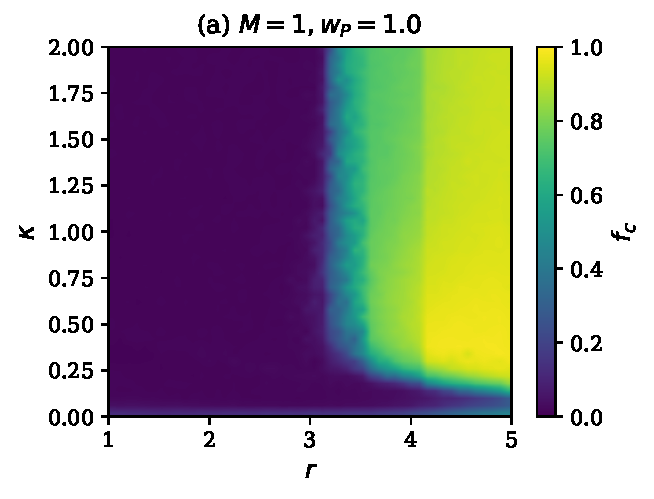
\includegraphics[width=0.49\linewidth]{figures/work1-original/Fig1a.pdf}\hfill
 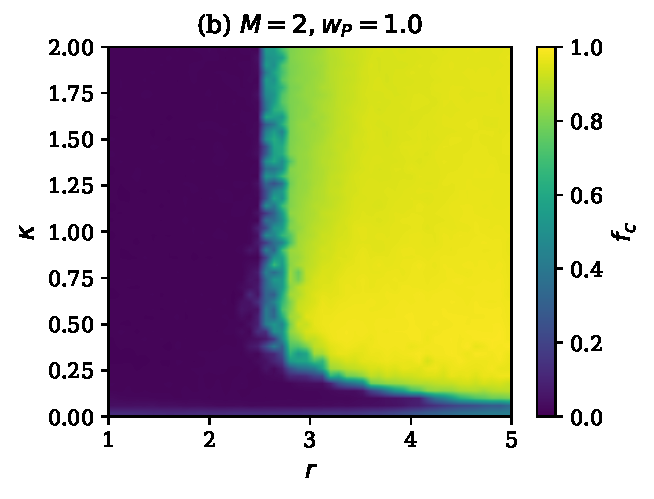
\includegraphics[width=0.49\linewidth]{figures/work1-original/Fig1b.pdf}
 \caption{协同因子 $r$ 与邻居影响强度 $\kappa$ 对合作率的共同影响，$w_P=1$。左、右分别为 $M=1$ 和 $M=2$；颜色表示合作率。}
 \label{fig:w1-kappa-map}
\par\smallskip{\zihao{-5}\rmfamily 来源：Kang等，文献\cite{kang2025neighbor}，2025年。\par}
\end{figure}

图\ref{fig:w1-kappa-dynamics}给出 $r=3.6$、$w_P=1$ 的时间演化比较。$\kappa=0$ 时合作率在初始波动后下降，加入 NI 后则出现先下降、后恢复的过程。在图示比较中，较大的影响强度使恢复更早出现；在相应条件下，$M=2$ 的恢复也早于 $M=1$。但曲线的后期排序不同：例如 $M=1$ 时，$\kappa=0.5$ 的后期合作率高于图中更大的 $\kappa$。因而，加快合作出现与提高最终合作水平之间存在需要分别评价的权衡。这一现象说明，NI 的影响体现在学习轨迹随时间的改变，而不仅是最终一个合作率数值的差别。初期合作下降与后期恢复可以同时存在，不能仅依据初期表现判断机制的长期作用。

\begin{figure}[htbp]
 \centering
 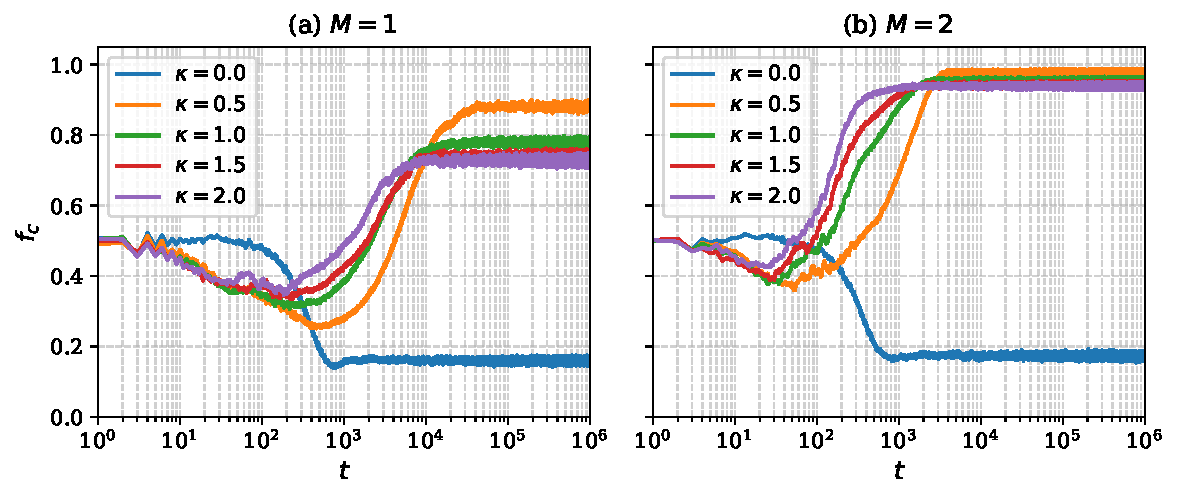
\includegraphics[width=\linewidth]{figures/work1-original/Figure_2.pdf}
 \caption{不同 $\kappa$ 下的合作率时间演化，$r=3.6$、$w_P=1$。左、右分别为 $M=1$ 和 $M=2$。更早恢复与更高的最终合作率是不同的评价维度。}
 \label{fig:w1-kappa-dynamics}
\par\smallskip{\zihao{-5}\rmfamily 来源：Kang等，文献\cite{kang2025neighbor}，2025年。\par}
\end{figure}

图\ref{fig:w1-lattice}的空间快照为上述动态提供了补充观察。在 $r=3.6$、$w_P=1$、$M=1$ 下，原研究比较了 $\kappa=0$ 与 $\kappa=0.5$ 在 $t=100,1000,10000$ 的策略分布。源稿描述，无 NI 时合作与背叛个体较为混杂；加入 NI 后，后期出现更清晰的合作聚集区域。这种空间组织与合作率恢复相对应，支持合作团簇形成的解释。但少量快照本身不能识别所有团簇边界事件，也不能单独证明局部奖励差是团簇扩张的唯一原因。

\begin{figure}[htbp]
 \centering
 \begin{tabular}{@{}c c c c@{}}
 & $t=100$ & $t=1000$ & $t=10000$\\
 $\kappa=0$ &
 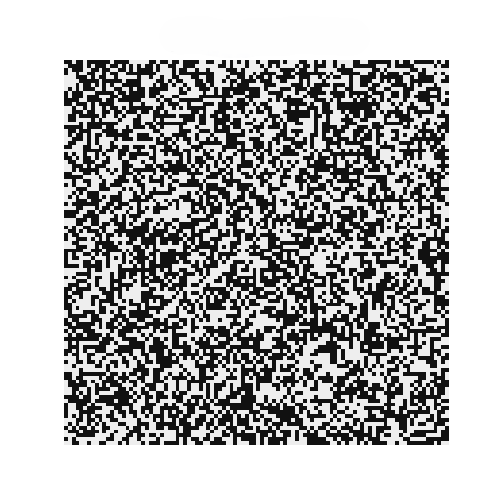
\includegraphics[width=0.27\linewidth]{figures/work1-original/lattice_k0_t100.png} &
 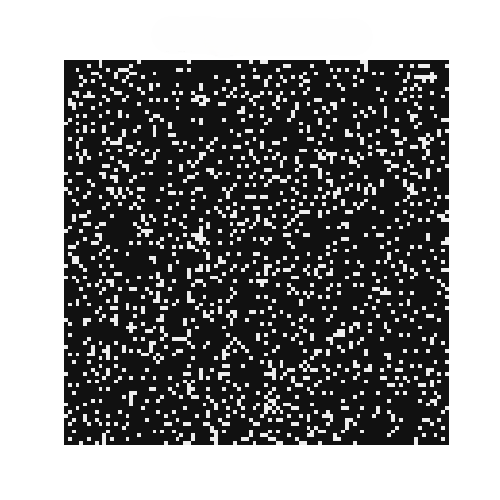
\includegraphics[width=0.27\linewidth]{figures/work1-original/lattice_k0_t1000.png} &
 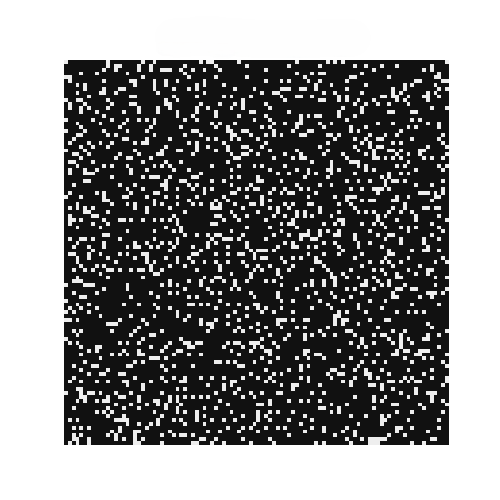
\includegraphics[width=0.27\linewidth]{figures/work1-original/lattice_k0_t10000.png}\\
 $\kappa=0.5$ &
 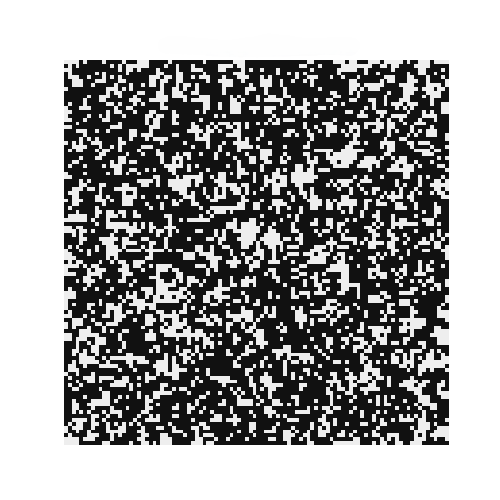
\includegraphics[width=0.27\linewidth]{figures/work1-original/lattice_k0.5_t100.png} &
 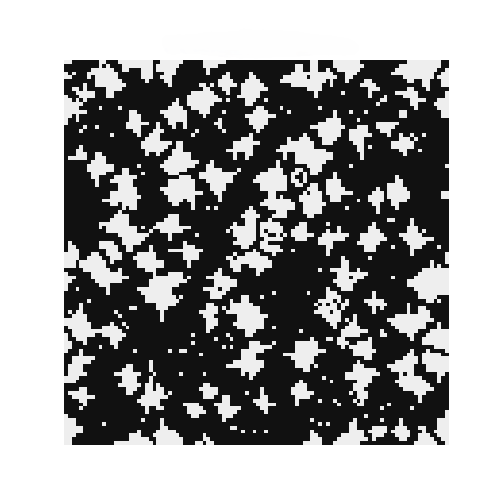
\includegraphics[width=0.27\linewidth]{figures/work1-original/lattice_k0.5_t1000.png} &
 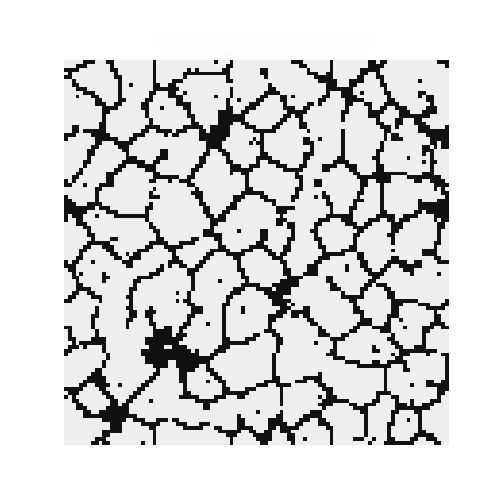
\includegraphics[width=0.27\linewidth]{figures/work1-original/lattice_k0.5_t10000.png}
 \end{tabular}
 \caption{NI 对策略空间分布的影响，$r=3.6$、$w_P=1$、$M=1$。浅灰色表示合作，黑色表示背叛；上、下两行分别为 $\kappa=0$ 和 $\kappa=0.5$。各快照按原始时间节点重新排版。}
 \label{fig:w1-lattice}
\par\smallskip{\zihao{-5}\rmfamily 来源：Kang等，文献\cite{kang2025neighbor}，2025年。\par}
\end{figure}

更新贡献分析进一步说明了标准学习与邻居修正的共同作用。图\ref{fig:w1-ni-share}显示，NI 的平均相对贡献在早期达到峰值，之后下降并保持持续波动；较大的 $\kappa$ 对应较大的贡献比例。随着动作和奖励分布变化，正奖励差及修正量也会变化，即使控制参数 $\kappa$ 固定，实际影响强度仍然随时间改变。这种由规则产生的动态变化，不意味着系统额外训练了一个影响强度控制器。

\begin{figure}[htbp]
 \centering
 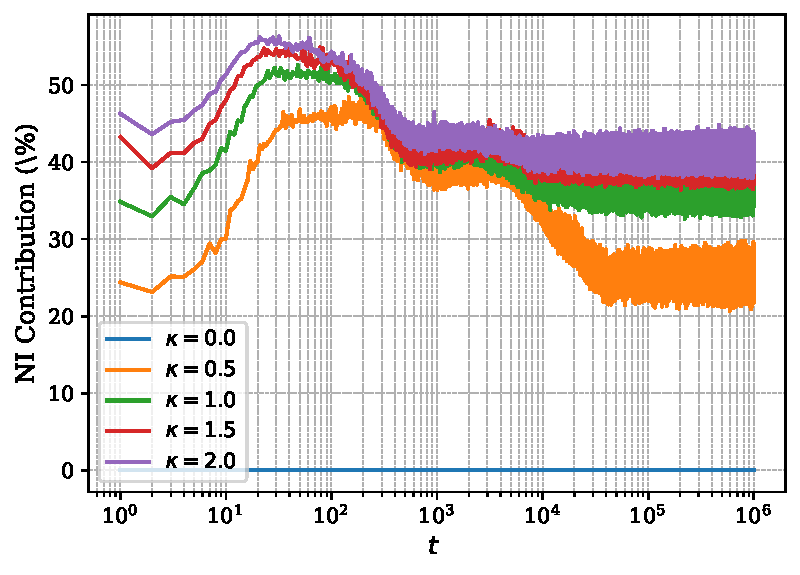
\includegraphics[width=0.78\linewidth]{figures/work1-original/Figure_4.pdf}
 \caption{NI 在 Q 值更新中的平均相对贡献，$r=3.6$、$w_P=1$、$M=1$。纵轴按式\eqref{eq:w1-ni-share}计算，表示更新幅度构成。}
 \label{fig:w1-ni-share}
\par\smallskip{\zihao{-5}\rmfamily 来源：Kang等，文献\cite{kang2025neighbor}，2025年。\par}
\end{figure}

\subsection{奖励组成及其与邻居影响的共同作用}

图\ref{fig:w1-reward-map}在 $\kappa=0$ 时通过改变 $w_P$ 考察直接声誉奖励的作用。源稿报告，当声誉奖励占有足够权重时，部分低协同因子条件下也能够维持较高合作；当 $w_P$ 接近1时，这种促进作用减弱。该结果与式\eqref{eq:w1-reward}一致：降低 $w_P$ 会提高合作动作的即时声誉奖励，使个体的学习目标发生变化。因此，此处的合作提高应与奖励设计联系起来解释，不能全部归因于空间信息传播。

\begin{figure}[htbp]
 \centering
 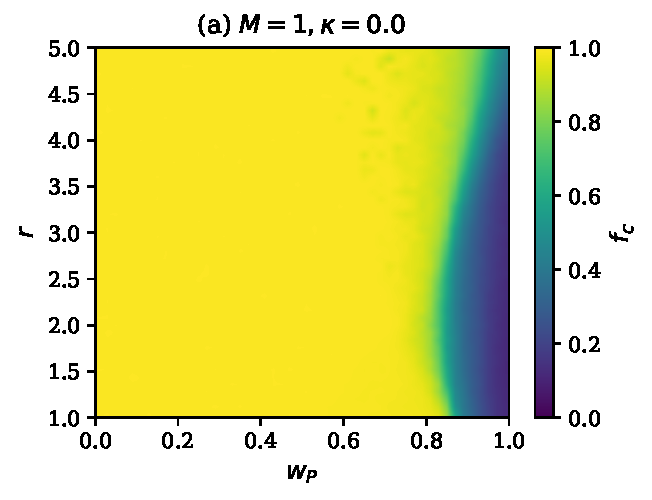
\includegraphics[width=0.49\linewidth]{figures/work1-original/Fig5a.pdf}\hfill
 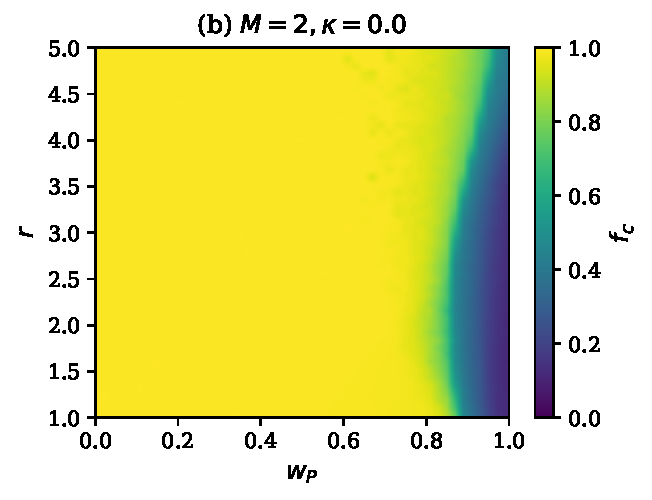
\includegraphics[width=0.49\linewidth]{figures/work1-original/Fig5b.pdf}
 \caption{博弈收益权重 $w_P$ 与协同因子 $r$ 对合作率的共同影响，$\kappa=0$。左、右分别为 $M=1$ 和 $M=2$。}
 \label{fig:w1-reward-map}
\par\smallskip{\zihao{-5}\rmfamily 来源：Kang等，文献\cite{kang2025neighbor}，2025年。\par}
\end{figure}

图\ref{fig:w1-reward-dynamics}进一步展示奖励权重与协同因子之间的非单调现象。在 $w_P=0.83$、$M=1$、$\kappa=0$ 的代表性比较中，$r=1.0$ 与 $r=2.0$ 的合作演化及合作者声誉奖励贡献不同。源稿将这一现象与声誉项在综合奖励中的相对作用联系起来。该解释提示，改变 $r$ 不仅改变原始博弈收益，也通过归一化和奖励组成影响学习信号。相关贡献曲线提供了机制线索，但尚不能替代对奖励组成进行独立控制的因果比较。

\begin{figure}[htbp]
 \centering
 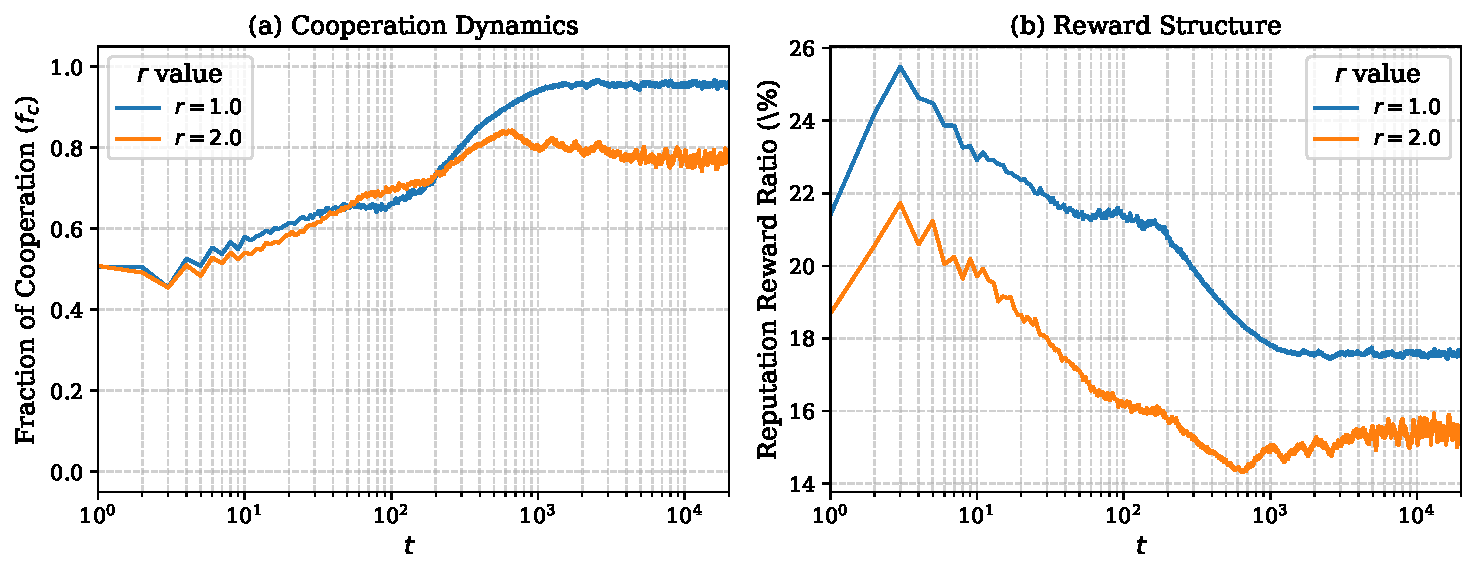
\includegraphics[width=\linewidth]{figures/work1-original/Figure_Reward_vs_Coop_SideBySide.pdf}
 \caption{奖励组成与非单调合作现象的对应关系，$w_P=0.83$、$M=1$、$\kappa=0$。左图为 $r=1.0$ 和 $r=2.0$ 的合作演化，右图为合作者综合奖励中声誉部分的平均相对贡献。}
 \label{fig:w1-reward-dynamics}
\par\smallskip{\zihao{-5}\rmfamily 来源：Kang等，文献\cite{kang2025neighbor}，2025年。\par}
\end{figure}

为观察两种机制共同启用后的表现，原研究在 $r=3.0$ 下比较了三种配置：直接声誉奖励配置 $(\kappa=0,w_P=0.95)$、NI 配置 $(\kappa=1,w_P=1)$，以及联合配置 $(\kappa=1,w_P=0.95)$。图\ref{fig:w1-hybrid}显示，联合配置在两种感知范围下均取得更好的合作形成表现。单独 NI 在 $M=1$ 时经历较长的低合作阶段，但后期仍发生恢复；因而不能将其概括为整个观察时段内始终无效。从机制上看，声誉奖励直接改变动作的即时回报，NI 则把邻居的相对综合奖励转换为价值修正，两者作用于学习过程的不同环节。

\begin{figure}[htbp]
 \centering
 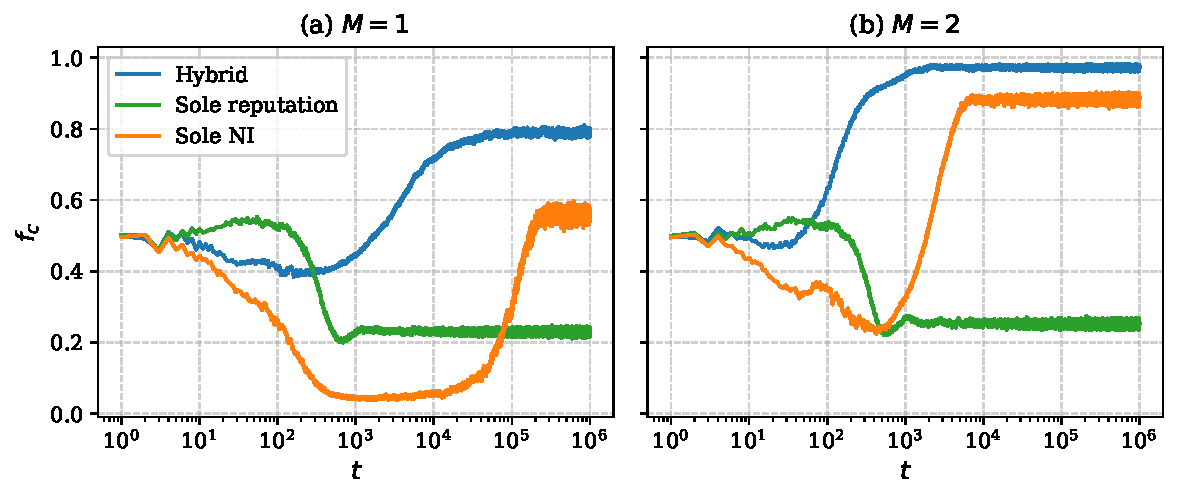
\includegraphics[width=\linewidth]{figures/work1-original/Figure_6.pdf}
 \caption{声誉奖励与 NI 单独或共同启用时的合作演化，$r=3.0$。直接声誉奖励：$(\kappa,w_P)=(0,0.95)$；NI：$(1,1)$；联合配置：$(1,0.95)$。左、右分别为 $M=1$ 和 $M=2$。}
 \label{fig:w1-hybrid}
\par\smallskip{\zihao{-5}\rmfamily 来源：Kang等，文献\cite{kang2025neighbor}，2025年。\par}
\end{figure}

这一比较支持两种机制在所测条件下具有互补作用。由于三条曲线本身不足以给出完整的交互效应估计，本章不进一步将其解释为已完成统计检验的超加性效应。另需注意，“单独声誉奖励”与“单独 NI”是对即时奖励和附加修正配置的简称，三种配置均保留式\eqref{eq:w1-state}的声誉状态。

声誉空间分布见图\ref{fig:w1-reputation-map}。在原图图注给出的 $r=3.6$、$M=1$ 条件下，联合配置形成了更大面积的高声誉聚集区域；单独 NI 也存在较小的高声誉区域。声誉反映累积行为，故该图需要结合动作分布理解，不能直接把任一声誉阈值当作当轮合作动作。

\begin{figure}[htbp]
 \centering
 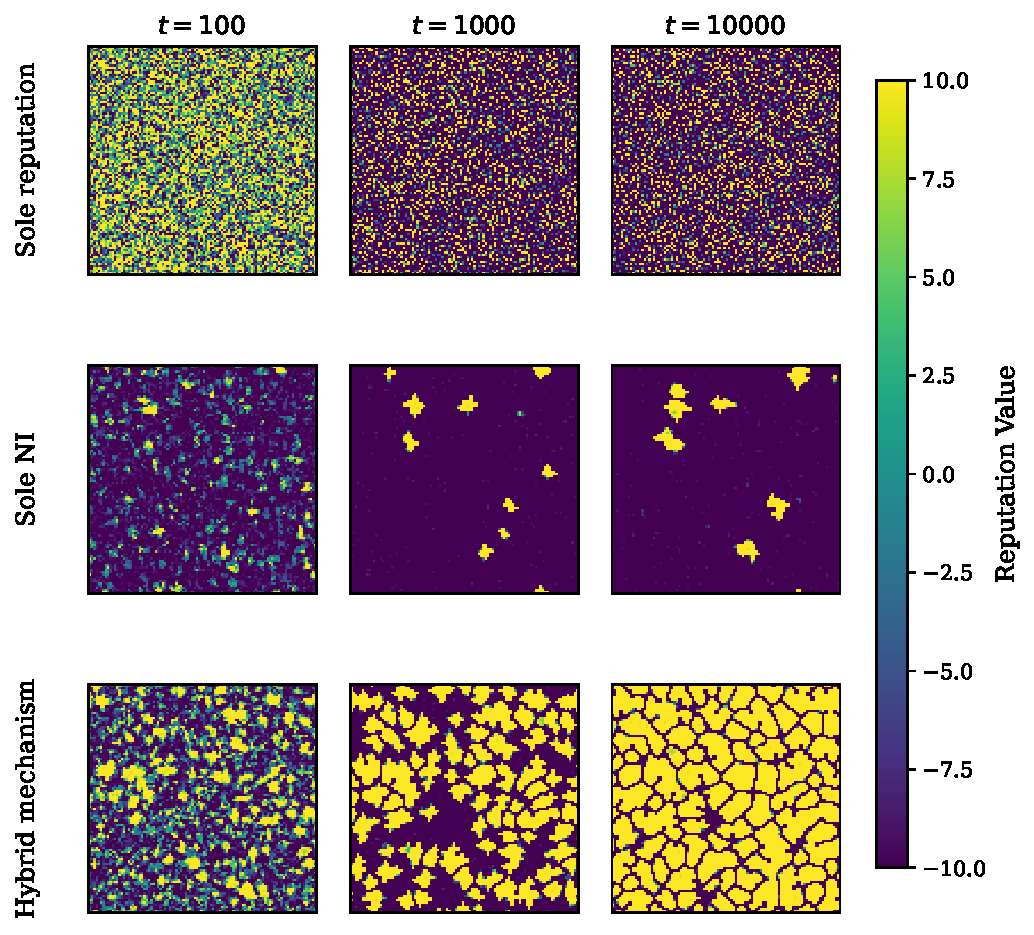
\includegraphics[width=0.72\linewidth]{figures/work1-original/Figure_7.pdf}
 \caption{三种配置的声誉空间分布。按原稿图注，$r=3.6$、$M=1$；从上到下依次为直接声誉奖励 $(0,0.95)$、NI $(1,1)$ 和联合配置 $(1,0.95)$，括号表示 $(\kappa,w_P)$。三列为 $t=100,1000,10000$，颜色表示声誉值。}
 \label{fig:w1-reputation-map}
\par\smallskip{\zihao{-5}\rmfamily 来源：Kang等，文献\cite{kang2025neighbor}，2025年。\par}
\end{figure}

\subsection{感知范围与邻居信息来源}

图\ref{fig:w1-range}比较 $r=3.0$、$w_P=0.95$ 下的两种感知范围。启用 NI 后，$M=2$ 相比 $M=1$ 能够加快合作形成并提高相应条件下的合作水平；关闭 NI 后，两种感知范围的表现差别较小。这说明所测条件下扩大感知范围的收益主要体现于邻居修正环节。由于 $M$ 同时改变状态所用的声誉集合和 NI 候选集合，这一实验并未完全分离两条信息路径，因而不能进一步断言状态路径在所有条件下均无作用。

\begin{figure}[htbp]
 \centering
 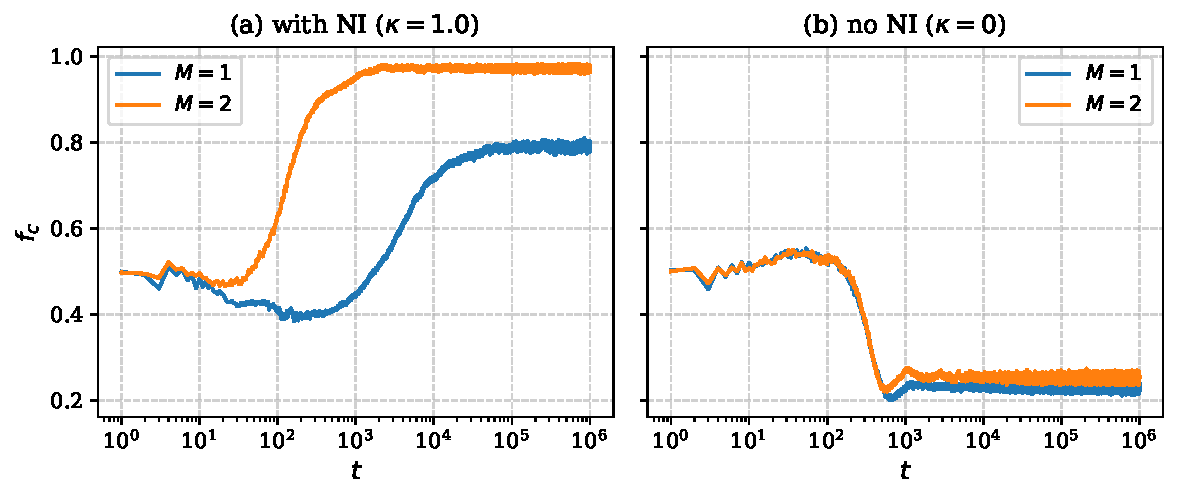
\includegraphics[width=\linewidth]{figures/work1-original/Figure_8.pdf}
 \caption{感知范围对合作演化的影响，$r=3.0$、$w_P=0.95$。左图启用 NI，$\kappa=1$；右图关闭 NI，$\kappa=0$。}
 \label{fig:w1-range}
\par\smallskip{\zihao{-5}\rmfamily 来源：Kang等，文献\cite{kang2025neighbor}，2025年。\par}
\end{figure}

为了解较远邻居是否被实际使用，原研究统计了 $M=2$ 时触发 NI 的参考对象来源。图\ref{fig:w1-second-order}中，二阶来源比例早期上升，后期下降并持续波动，主要位于约 $55\%$--$72.5\%$ 的范围，个别波动超出该区间。这一观测说明二阶邻居确实参与了价值修正，而不是只出现在名义感知集合中。但候选集合本身包含八个二阶邻居和四个一阶邻居，按候选数均匀选择时，二阶比例即为 $8/12\approx66.7\%$。因此，“占多数”不能单独证明模型对二阶邻居存在超出候选数量差异的偏好。若需判断这种偏好，还应结合候选机会、正奖励优势条件和并列最高奖励的处理方式建立对照。

\begin{figure}[htbp]
 \centering
 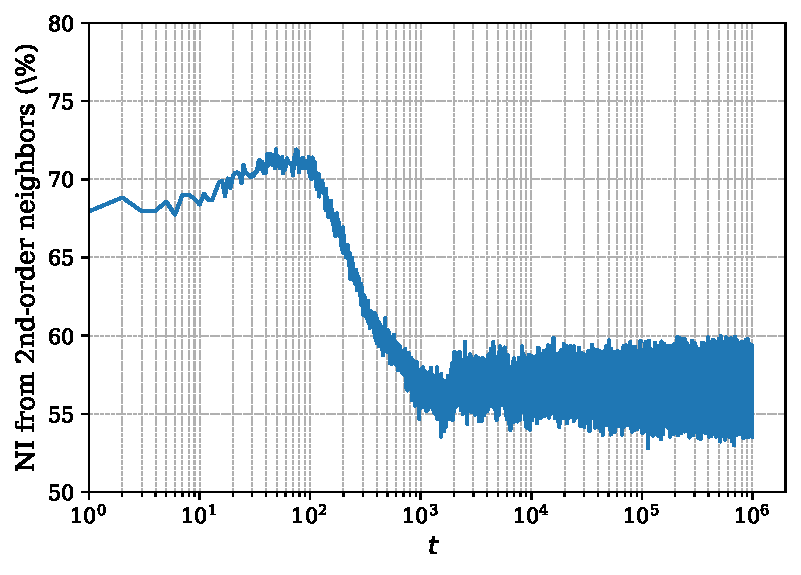
\includegraphics[width=0.78\linewidth]{figures/work1-original/Figure_9.pdf}
 \caption{触发 NI 的参考对象中二阶邻居所占比例，$r=3.0$、$\kappa=1$、$w_P=0.95$、$M=2$。纵轴统计参考来源，不表示合作率或异常识别率。}
 \label{fig:w1-second-order}
\par\smallskip{\zihao{-5}\rmfamily 来源：Kang等，文献\cite{kang2025neighbor}，2025年。\par}
\end{figure}

从计算机制看，扩大候选集合可能使智能体获得原一阶集合之外的相对表现信息。在奖励真实的前提下，这为个体提供了更多参考机会；但更大的集合并不保证参考对象一定有助于合作，因为 NI 同样可能强化具有奖励优势的背叛动作。感知范围的收益仍取决于相应环境中的动作和奖励结构。

\subsection{状态表示与策略切换}

原论文还在 $r=4.6$、$w_P=1$、$\kappa=0$、$M=1$ 下比较了两种状态表示：以邻域平均声誉构造状态，以及以个体上一轮动作为状态。图\ref{fig:w1-stability}显示，声誉状态的策略切换较少，但后期合作率也低于动作状态。这里体现了行为稳定性与合作水平之间的权衡，不能将切换减少直接等同于所有性能均得到改善。这一结果表明，合作水平与行为稳定性是不同的观测维度；最终合作率相近的系统，其逐轮动作变化仍可能不同。

若以
\begin{equation}
 n_{\mathrm{sw}}(t)=\sum_{i\in\mathcal V}\mathbb I\{a_i(t)\neq a_i(t-1)\}
 \label{eq:w1-switch}
\end{equation}
表示每轮切换个体数，则 $n_{\mathrm{sw}}(t)/N_{\mathrm{tot}}$ 是对应切换率。引用原论文结果时需区分这两种尺度，避免把数量曲线写成比例曲线。较少切换说明在所测条件下行为变化较少，但并不等价于对消息故障具有鲁棒性，也不构成最优策略收敛的证明。

\begin{figure}[htbp]
 \centering
 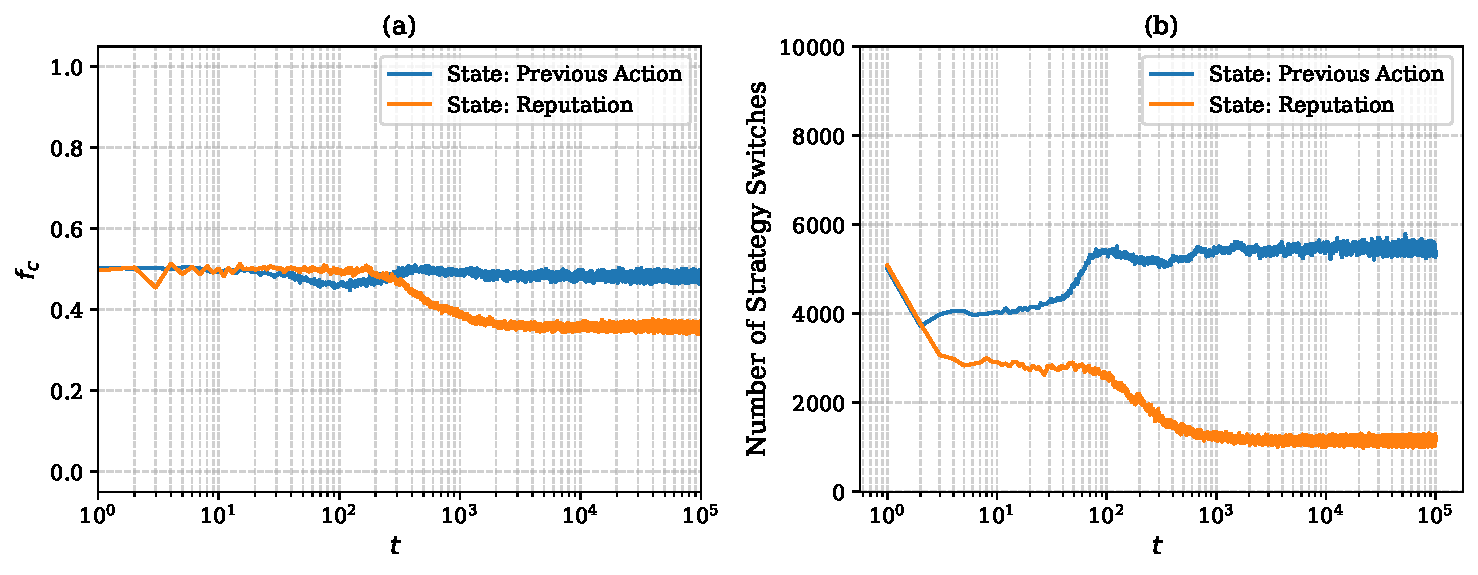
\includegraphics[width=\linewidth]{figures/work1-original/Figure_Coop_vs_Stability_Comparison.pdf}
 \caption{声誉状态与上一轮动作状态的比较，$r=4.6$、$w_P=1$、$\kappa=0$、$M=1$。左图为合作率，右图为每轮策略切换个体数。}
 \label{fig:w1-stability}
\par\smallskip{\zihao{-5}\rmfamily 来源：Kang等，文献\cite{kang2025neighbor}，2025年。\par}
\end{figure}

\section{本章小结与研究边界}

本章介绍了基于邻居相对表现的合作促进机制。智能体在自身 Q-learning 更新之后，参考局部候选集合中综合奖励更高的邻居，并按照动作一致性修正已执行动作的 Q 值。该方法保留个体价值表和探索决策过程，通过附加更新使邻居经验参与价值判断。原研究的结果表明，在相应博弈参数下，这一机制能够改变合作演化轨迹，并伴随更清晰的合作聚集；奖励组成与感知范围进一步影响其作用。

这些结果也界定了方法的适用边界。NI 使用固定的奖励排序与修正规则，优先选择观测值最高的候选对象，未评估消息来源的可信程度。影响强度虽然随相对奖励差变化，但其调节依据仍是同一组被假设为真实的观测。当邻居报告失真时，参考对象和修正幅度可能同时受到影响。由此，后续研究将信息条件从可靠观测扩展到可能失真的邻居消息，进一步研究参考对象选择与影响强度控制，并在明确的异常模型下评价其效果。
